% This file was created by tikzplotlib v0.9.4.
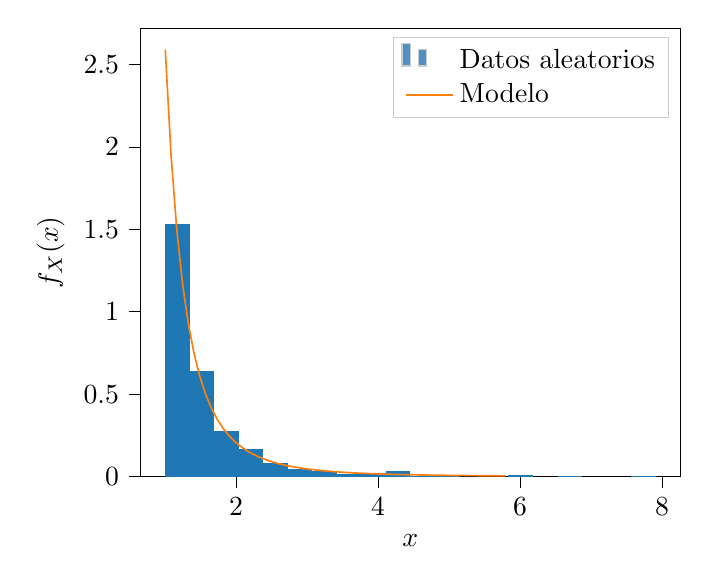
\begin{tikzpicture}

\definecolor{color0}{rgb}{0.12156862745098,0.466666666666667,0.705882352941177}
\definecolor{color1}{rgb}{1,0.498039215686275,0.0549019607843137}

\begin{axis}[
legend cell align={left},
legend style={fill opacity=0.8, draw opacity=1, text opacity=1, draw=white!80!black},
tick align=outside,
tick pos=left,
x grid style={white!69.0196078431373!black},
xlabel={\(\displaystyle x\)},
xmin=0.654797278306265, xmax=8.25687545466215,
xtick style={color=black},
y grid style={white!69.0196078431373!black},
ylabel={\(\displaystyle f_X(x)\)},
ymin=0, ymax=2.71986951576802,
ytick style={color=black}
]
\draw[draw=none,fill=color0] (axis cs:1.00034628632244,0) rectangle (axis cs:1.34589529433862,1.53379111994206);
\addlegendimage{ybar,ybar legend,draw=none,fill=color0};
\addlegendentry{Datos aleatorios}

\draw[draw=none,fill=color0] (axis cs:1.34589529433862,0) rectangle (axis cs:1.69144430235479,0.642455903070071);
\draw[draw=none,fill=color0] (axis cs:1.6914443023548,0) rectangle (axis cs:2.03699331037097,0.277818768895166);
\draw[draw=none,fill=color0] (axis cs:2.03699331037097,0) rectangle (axis cs:2.38254231838715,0.167848839540829);
\draw[draw=none,fill=color0] (axis cs:2.38254231838715,0) rectangle (axis cs:2.72809132640333,0.08103047426109);
\draw[draw=none,fill=color0] (axis cs:2.72809132640332,0) rectangle (axis cs:3.0736403344195,0.0463031281491944);
\draw[draw=none,fill=color0] (axis cs:3.0736403344195,0) rectangle (axis cs:3.41918934243568,0.0347273461118957);
\draw[draw=none,fill=color0] (axis cs:3.41918934243568,0) rectangle (axis cs:3.76473835045186,0.0173636730559479);
\draw[draw=none,fill=color0] (axis cs:3.76473835045185,0) rectangle (axis cs:4.11028735846803,0.0231515640745971);
\draw[draw=none,fill=color0] (axis cs:4.11028735846803,0) rectangle (axis cs:4.45583636648421,0.0347273461118958);
\draw[draw=none,fill=color0] (axis cs:4.45583636648421,0) rectangle (axis cs:4.80138537450038,0.0057878910186493);
\draw[draw=none,fill=color0] (axis cs:4.80138537450038,0) rectangle (axis cs:5.14693438251656,0.0057878910186493);
\draw[draw=none,fill=color0] (axis cs:5.14693438251656,0) rectangle (axis cs:5.49248339053274,0);
\draw[draw=none,fill=color0] (axis cs:5.49248339053274,0) rectangle (axis cs:5.83803239854891,0);
\draw[draw=none,fill=color0] (axis cs:5.83803239854891,0) rectangle (axis cs:6.18358140656509,0.0115757820372986);
\draw[draw=none,fill=color0] (axis cs:6.18358140656509,0) rectangle (axis cs:6.52913041458127,0);
\draw[draw=none,fill=color0] (axis cs:6.52913041458127,0) rectangle (axis cs:6.87467942259744,0.0057878910186493);
\draw[draw=none,fill=color0] (axis cs:6.87467942259744,0) rectangle (axis cs:7.22022843061362,0);
\draw[draw=none,fill=color0] (axis cs:7.22022843061362,0) rectangle (axis cs:7.5657774386298,0);
\draw[draw=none,fill=color0] (axis cs:7.5657774386298,0) rectangle (axis cs:7.91132644664597,0.00578789101864928);
\addplot [semithick, color1]
table {%
1.00384337293896 2.59035191977907
1.08511849727253 1.9468807621506
1.1663936216061 1.4935849317286
1.24766874593966 1.16636800184441
1.32894387027323 0.925096039082917
1.4102189946068 0.743851178458825
1.49149411894036 0.60543753015758
1.57276924327393 0.498170530613812
1.6540443676075 0.413940252763476
1.73531949194106 0.347009850052935
1.81659461627463 0.293251117969427
1.8978697406082 0.249647039940814
1.97914486494176 0.213961392467284
2.06041998927533 0.184515196635756
2.1416951136089 0.160032879983694
2.22297023794246 0.139534755106771
2.30424536227603 0.122260790053532
2.3855204866096 0.107615847165405
2.46679561094316 0.0951298615860002
2.54807073527673 0.0844285539319274
2.6293458596103 0.0752116622067165
2.71062098394386 0.0672366024854644
2.79189610827743 0.0603060910669847
2.873171232611 0.0542586863597021
2.95444635694456 0.0489615029469722
3.03572148127813 0.0443045559627437
3.1169966056117 0.0401963392682552
3.19827172994526 0.03656034468851
3.27954685427883 0.0333323043519244
3.3608219786124 0.0304579925595032
3.44209710294596 0.0278914634944682
3.52337222727953 0.0255936305713215
3.6046473516131 0.0235311151922027
3.68592247594666 0.0216753091647893
3.76719760028023 0.0200016074939347
3.84847272461379 0.0184887777353072
3.92974784894736 0.0171184393526537
4.01102297328093 0.0158746321057419
4.09229809761449 0.0147434568218125
4.17357322194806 0.0137127752720289
4.25484834628163 0.0127719585115414
4.33612347061519 0.0119116751166727
4.41739859494876 0.0111237123931667
4.49867371928233 0.010400824932428
4.57994884361589 0.00973660593226292
4.66122396794946 0.00912537753162539
4.74249909228303 0.00856209707909922
4.82377421661659 0.00804227679625721
4.90504934095016 0.00756191473607643
4.98632446528373 0.00711743529392869
5.06759958961729 0.00670563782055226
5.14887471395086 0.00632365212565753
5.23014983828443 0.00596889985757352
5.31142496261799 0.00563906090667402
5.39270008695156 0.00533204411467232
5.47397521128513 0.005045961683401
5.55525033561869 0.00477910676954682
5.63652545995226 0.00452993382933617
5.71780058428583 0.00429704134207237
5.79907570861939 0.00407915659591138
};
\addlegendentry{Modelo}
\end{axis}

\end{tikzpicture}
